%
% Diplomarbeit mit LaTeX
% ===========================================================================
% This is part of the book "Diplomarbeit mit LaTeX".
% Copyright (c) 2002, 2003, 2005 Tobias Erbsland, Andreas Nitsch
% See the file main.tex for copying conditions.
%

\chapter{Konfiguration}
\index{Konfiguration}

\section{MiKTeX}
\index{Konfiguration!MiKTeX}

Die \DMLLaTeX-Distribution \enquote{MiKTeX} musst du nicht konfigurieren. Es handelt sich dabei au�er bei dem DVI-Betrachter um Kommandozeilentools. Du solltest nur den Editor TeXnicCenter einrichten (siehe dazu \ref{sec:KonfigurationTeXnicCenter}).

Du solltest jedoch mit dem \enquote{MiKTeX Update Wizard} alle Pakete der Distribution auf den neuesten Stand zu bringen. Wie du das machst beschreibt die Hilfe zu MiKTeX ausf�hrlich\footnote{\enquote{User Guide}$\Rightarrow$\enquote{Maintenance}$\Rightarrow$\enquote{Installing Updates}}.

\section{TeXnicCenter}
\label{sec:KonfigurationTeXnicCenter}
\index{Konfiguration!TeXnicCenter}

\subsection{TeXnicCenter f�r die Verwendung mit MiKTeX konfigurieren}

Nach dem ersten Start erscheint der Einrichtungsassistent. Falls du diesen bereits abgebrochen hast, kann man Ihn �ber das Men� \enquote{Ausgabe}, \enquote{Ausgabeprofile definieren...} und dort in dem Dialog \enquote{Assistent} links unten erneut aufrufen. Doch wie schon gesagt, der Assistent startet normalerweise beim ersten Start vom TeXnicCenter automatisch.

\begin{figure}[hb]
	\begin{captionbeside}[Start des Konfigurations-Assistenten]{Der Assistent Startet mit dem diesem Screen}[l]
		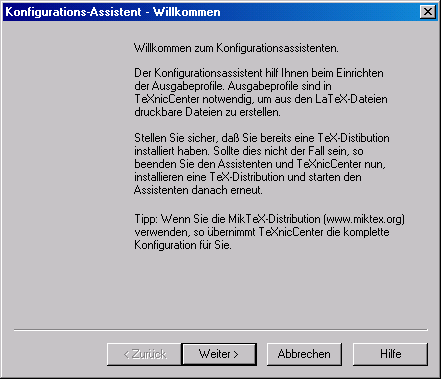
\includegraphics[width=7cm]{images/konfiguration01.png}
	\end{captionbeside}
	\label{fig:konfiguration01}
\end{figure}

\begin{figure}[hb]
	\begin{captionbeside}[Frage, f�r welche Distribution TeXnicCenter eingerichtet werden soll]{Hier teilt dir der Installationsassistent mit, dass er die installierte \enquote{MiKTeX}-Distribution erkannt hat und fragt, ob er den Editor mit dieser \DMLLaTeX-Distribution konfigurieren soll. Du w�hlst nat�rlich \enquote{Ja}.}[l]
		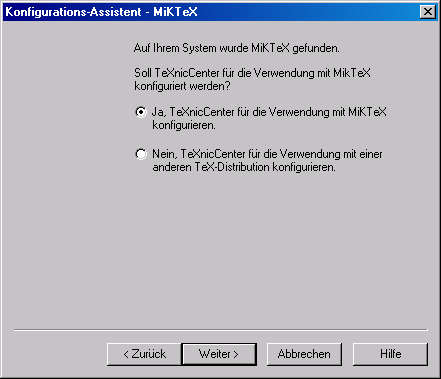
\includegraphics[width=7cm]{images/konfiguration02.png}
	\end{captionbeside}
	\label{fig:konfiguration02}
\end{figure}

\begin{figure}[ht]
	\begin{captionbeside}[Optionale Eingabe eines Postscript Betrachters]{Jetzt wirst du nach einem Programm zur PostScript-Betrachtung gefragt. Hier l�sst du alle Felder leer.}[l]
		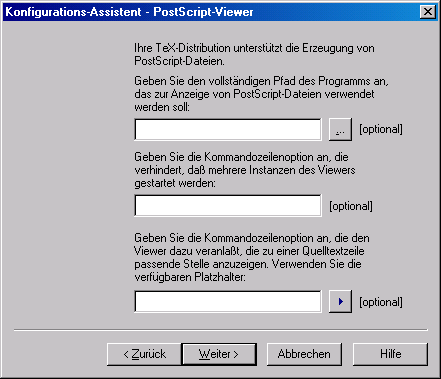
\includegraphics[width=7cm]{images/konfiguration03.png}
	\end{captionbeside}
	\label{fig:konfiguration03}
\end{figure}

\begin{figure}[ht]
	\begin{captionbeside}[Anzeige der drei generierten Profile]{Der TeXnicCenter-Assistent teilt dir mit, das er drei Profile generieren wird. Ein DVI-, ein PostScript- und ein PDF-Profil. Wir werden nur das PDF-Profil verwenden.}[l]
		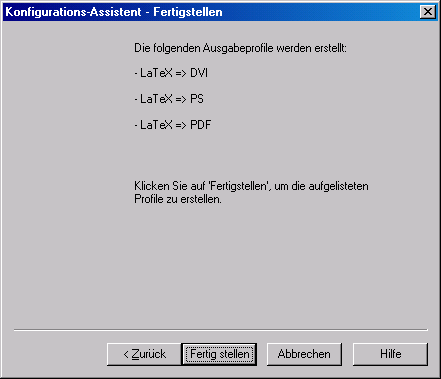
\includegraphics[width=7cm]{images/konfiguration04.png}
	\end{captionbeside}
	\label{fig:konfiguration04}
\end{figure}

\clearpage % Warten auf alle Floats

\subsection{Die Rechtschreibpr�fung}
\index{Rechtschreibprufung@Rechtschreibpr�fung}

Ein sehr sch�nes und n�tzliches Feature, welches dir TeXnicCenter bietet ist die Rechtschreibpr�fung. W�hle dazu im Men� \emph{Extras} den Punkt \emph{Optionen} aus. In dem Dialog, der sich ge�ffnet hat w�hlst du den Reiter \emph{Rechtschreibung} aus. Dort kannst du die verschiedenen Optionen der Rechtschreibpr�fung einstellen.

Die m�glichen Einstellparameter sind selbsterkl�rend, was du sehr gut in Abbildung \ref{fig:rechtschreibung} siehst.

\begin{figure}
	\centering
		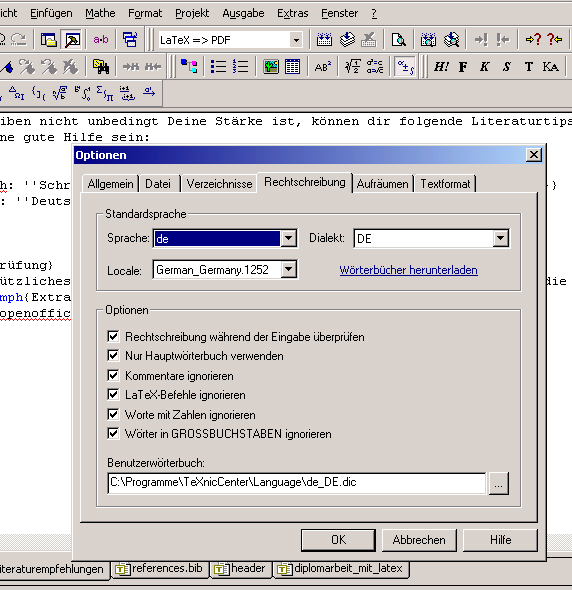
\includegraphics[width=0.60\textwidth]{images/rechtschreibung.png}
	\caption{Konfigurationsm�glichkeiten der Rechtschreibpr�fung}
	\label{fig:rechtschreibung}
\end{figure}

Falls eine gew�nschte Sprache fehlt, kannst du zus�tzliche W�rterb�cher installieren. W�rterb�cher diverser Sprachen, auch der neuen und alten deutschen Rechtschreibung, findest du unter folgender Internetadresse zum kostenlosen Download:

\url{http://lingucomponent.openoffice.org/download\_dictionary.html}

Entpacke die in der heruntergeladenen ZIP Datei enthaltenen Dateien in das Unterverzeichnis \enquote{Language} deiner TeXnicCenter Installation. Die TeXnicCenter Installation findest du normalerweise in dem folgenden Verzeichnis:

\verb|C:\Programme\TeXnicCenter\Language|



